%package list
\documentclass{article}
\usepackage[top=3cm, bottom=3cm, outer=3cm, inner=3cm]{geometry}
\usepackage{multicol}
\UseRawInputEncoding
\usepackage{graphicx}
\usepackage{url}
%\usepackage{cite}
\usepackage{hyperref}
\usepackage{array}
%\usepackage{multicol}
\newcolumntype{x}[1]{>{\centering\arraybackslash\hspace{0pt}}p{#1}}
\usepackage{natbib}
\usepackage{pdfpages}
\usepackage{multirow}
\usepackage[normalem]{ulem}
\useunder{\uline}{\ul}{}
\usepackage{svg}
\usepackage{xcolor}
\usepackage{listings}
\lstdefinestyle{ascii-tree}{
    literate={├}{|}1 {─}{--}1 {└}{+}1
  }
\lstset{basicstyle=\ttfamily,
  showstringspaces=false,
  commentstyle=\color{red},
  keywordstyle=\color{blue}
}
%\usepackage{booktabs}
\usepackage{caption}
\usepackage{subcaption}
\usepackage{float}
\usepackage{array}

\newcolumntype{M}[1]{>{\centering\arraybackslash}m{#1}}
\newcolumntype{N}{@{}m{0pt}@{}}

%------------------------------ ÍTEMS ------------------------------

\newcommand{\itemEmail}{hchoquehuancaz@unsa.edu.pe}
\newcommand{\itemStudent}{Hernan Andy Choquehuanca Zapana}
\newcommand{\itemCourse}{Fundamentos de la Programacion II}
\newcommand{\itemCourseCode}{20232191}
\newcommand{\itemSemester}{II}
\newcommand{\itemUniversity}{Universidad Nacional de San Agustin de Arequipa}
\newcommand{\itemFaculty}{Facultad de Ingenieria de Produccion y Servicios}
\newcommand{\itemDepartment}{Departamento Academico de Ingenieria de Sistemas e Informatica}
\newcommand{\itemSchool}{Escuela Profesional de Ingenieria de Sistemas}
\newcommand{\itemAcademic}{2023 - B}
\newcommand{\itemInput}{Del 11 Octubre 2023}
\newcommand{\itemOutput}{Al 16 Octubre 2023}
\newcommand{\itemPracticeNumber}{06}
\newcommand{\itemTheme}{ArrayList}

%------------------------------  ------------------------------

\usepackage[english,spanish]{babel}
\usepackage[utf8]{inputenc}
\AtBeginDocument{\selectlanguage{Spanish}}
\renewcommand{\figurename}{Figura}
\renewcommand{\refname}{Referencias}
\renewcommand{\tablename}{Tabla} %esto no funciona cuando se usa babel
\AtBeginDocument{
	\renewcommand\tablename{Tabla}
}

\usepackage{fancyhdr}
\pagestyle{fancy}
\fancyhf{}
\setlength{\headheight}{30pt}
\renewcommand{\headrulewidth}{1pt}
\renewcommand{\footrulewidth}{1pt}
\fancyhead[L]{\raisebox{-0.2\height}{
\includegraphics[width=3cm]{img/logo_episunsa.png}}}
\fancyhead[C]{\fontsize{7}{7}\selectfont	\itemUniversity \\ \itemFaculty \\ \itemDepartment \\ \itemSchool \\ \textbf{\itemCourse}}
\fancyhead[R]{\raisebox{-0.2\height}{
\includegraphics[width=1.2cm]{img/logo_abet}}}
\fancyfoot[L]{Estudiante: Hernan Choquehuanca Zapana}
\fancyfoot[R]{\itemCourse}
\fancyfoot[C]{Página \thepage}

% para el codigo fuente
\usepackage{listings}
\usepackage{color, colortbl}
\definecolor{dkgreen}{rgb}{0,0.6,0}
\definecolor{gray}{rgb}{0.5,0.5,0.5}
\definecolor{mauve}{rgb}{0.58,0,0.82}
\definecolor{codebackground}{rgb}{0.95, 0.95, 0.92}
\definecolor{tablebackground}{rgb}{0.8, 0, 0}

\lstset{frame=tb,
	language=bash,
	aboveskip=3mm,
	belowskip=3mm,
	showstringspaces=false,
	columns=flexible,
	basicstyle={\small\ttfamily},
	numbers=none,
	numberstyle=\tiny\color{gray},
	keywordstyle=\color{blue},
	commentstyle=\color{dkgreen},
	stringstyle=\color{mauve},
	breaklines=true,
	breakatwhitespace=true,
	tabsize=3,
	backgroundcolor= \color{codebackground},
}

%------------------------------ INICIO DEL DOCUMENTO------------------------------

\begin{document}
	
	\vspace*{10px}
	
	\begin{center}	
		\fontsize{17}{17} \textbf{ Informe de Laboratorio \itemPracticeNumber}
	\end{center}
	\centerline{\textbf{\Large Tema: \itemTheme}}
	%\vspace*{0.5cm}	

	\begin{flushright}
		\begin{tabular}{|M{2.5cm}|N|}
			\hline 
			\rowcolor{tablebackground}
			\color{white} \textbf{Nota}  \\
			\hline 
			     \\[30pt]
			\hline 			
		\end{tabular}
	\end{flushright}	

	\begin{table}[H]
		\begin{tabular}{|x{4.7cm}|x{4.8cm}|x{4.8cm}|}
			\hline 
			\rowcolor{tablebackground}
			\color{white} \textbf{Estudiante} & \color{white}\textbf{Escuela}  & \color{white}\textbf{Asignatura}   \\
			\hline 
			{\itemStudent \par \itemEmail} & \itemSchool & {\itemCourse \par Semestre: \itemSemester \par Código: \itemCourseCode}     \\
			\hline 			
		\end{tabular}
	\end{table}		
	
	\begin{table}[H]
		\begin{tabular}{|x{4.7cm}|x{4.8cm}|x{4.8cm}|}
			\hline 
			\rowcolor{tablebackground}
			\color{white}\textbf{Laboratorio} & \color{white}\textbf{Tema}  & \color{white}\textbf{Duración}   \\
			\hline 
			\itemPracticeNumber & \itemTheme & 02 horas   \\
			\hline 
		\end{tabular}
	\end{table}
	
	\begin{table}[H]
		\begin{tabular}{|x{4.7cm}|x{4.8cm}|x{4.8cm}|}
			\hline 
			\rowcolor{tablebackground}
			\color{white}\textbf{Semestre académico} & \color{white}\textbf{Fecha de inicio}  & \color{white}\textbf{Fecha de entrega}   \\
			\hline 
			\itemAcademic & \itemInput &  \itemOutput  \\
			\hline 
		\end{tabular}
	\end{table}


%------------------------------ ACTIVIDADES (TAREA) ------------------------------

	\section{Tarea}
	\begin{itemize}		
        \item Cree un Proyecto llamado Laboratorio6
        \item Usted deberá crear las dos clases Soldado.java y VideoJuego3.java. Puede reutilizar lo desarrollado en Laboratorios anteriores.
        \item Del Soldado nos importa el nombre, puntos de vida, fila y columna (posición en el tablero).
        \item El juego se desarrollará en el mismo tablero de los laboratorios anteriores. Pero ahora el tablero debe ser un ArrayList bidimensional.
        \item Tendrá 2 Ejércitos. Inicializar el tablero con n soldados aleatorios entre 1 y 10 para cada Ejército. Cada soldado tendrá un nombre autogenerado: Soldado0X1, Soldado1X1, etc., un valor de puntos de vida autogenerado aleatoriamente [1..5], la fila y columna también autogenerados aleatoriamente (no puede haber 2 soldados en el mismo cuadrado). Se debe mostrar el tablero con todos los soldados creados (distinguir los de un ejército de los del otro ejército). Además de los datos del Soldado con mayor vida de cada ejército, el promedio de puntos de vida de todos los soldados creados por ejército, los datos de todos los soldados por ejército en el orden que fueron creados y un ranking de poder de todos los soldados creados por ejército (del que tiene más nivel de vida al que tiene menos) usando 2 diferentes algoritmos de ordenamiento. Finalmente, que muestre qué ejército ganará la batalla (indicar la métrica usada para decidir al ganador de la batalla).

	\end{itemize}
		
	\section{Equipos, materiales y temas utilizados}
	\begin{itemize}
		\item Sistema Operativo Windows 11 Pro 22H2 64 bits.
		\item VIM 9.0.
		\item Visual Studio Code.
		\item Git 2.42.0.
		\item Cuenta en GitHub con el correo institucional.
        \item Variables Simples
        \item Métodos.
        \item Métodos de Búsqueda y Ordenamiento.
        \item ArrayList
        
	\end{itemize}
	
	\section{URL de Repositorio Github}
	\begin{itemize}
		\item URL del Repositorio GitHub para clonar o recuperar.
        \item \url{https://github.com/hernanchoquehuanca/fp2-23b.git}
		\item URL para el laboratorio 04 en el Repositorio GitHub.
		\item \url{https://github.com/hernanchoquehuanca/fp2-23b/tree/main/fase02/lab06}
	\end{itemize}
	
	\section{Trabajo del Laboratorio 06}
        
        
%-----------------------------------------------------------------------------------
%------------------------------------- ACTIVIDADES  --------------------------------
%-----------------------------------------------------------------------------------

% ACTIVIDADESSSS

    \subsection{Actividad 01}
    
        \subsubsection{Clase Soldado.java}
        \begin{itemize}	
            \item Haciendo uso de la clase Soldado.java del laboratorio anterior (lab05), se adaptó al ejercicio actual.
            \begin{itemize}
                \item Primero copiamos el código tal cual a la carpeta del laboratorio actual (lab06).
            \end{itemize}
            \item Nuestra clase Soldado tendrá los siguientes atributos:
            \begin{itemize}
                \item name (Nombre).
                \item row (Fila).
                \item column (Columna).
                \item status (Estado).
                \item health (Vida).
            \end{itemize}
            
        \end{itemize}
        \lstinputlisting[language=Java, firstline=2, lastline=6, firstnumber=2,numbers=left,]{src/Soldado.java}

        \begin{itemize}
            \item Además creamos el método constructor, tendiendo en cuenta que tiene que tener el mismo nombre que la clase y considerando sus atributos como parámetros:
            \begin{itemize}
                \item Se utilizó el puntero \textcolor{blue}{this} para evitar ambigüedades.
            \end{itemize}
        \end{itemize}

        \lstinputlisting[language=Java, firstline=8, lastline=14, firstnumber=8,numbers=left,]{src/Soldado.java}

        \begin{itemize}
            \item Luego de ello también se implementaron los getters y setters para cada atributo de nuestra clase Soldado.
            \begin{itemize}
                \item Setters: 
            \end{itemize}
        \end{itemize}

        \lstinputlisting[language=Java, firstline=16, lastline=30,firstnumber=16,numbers=left]{src/Soldado.java}

        \begin{itemize}
            \begin{itemize}
                \item Getters: 
            \end{itemize}
        \end{itemize}

        \lstinputlisting[language=Java, firstline=32, lastline=46,firstnumber=32,numbers=left]{src/Soldado.java}

        \begin{itemize}
            \item Y finalizando con esta clase, se creo el método toString().
            \begin{itemize}
                \item Se agregó la anotación \textcolor{blue}{@Override} para indicar que se está reemplazando el método de su clase padre \textcolor{blue}{Objetct}.
                \item En este método se considera los atributos de la clase (name, row, column, status, health).
                \item Se utilizaron saltos de con ayuda del \textcolor{blue}{\textbackslash n}.
            \end{itemize}
        \end{itemize}

        \lstinputlisting[language=Java, firstline=47, lastline=56,firstnumber=47,numbers=left]{src/Soldado.java}

        \begin{itemize}
            \begin{itemize}
                \item Un ejemplo de como se muestra en la siguiente imagen:
            \end{itemize}
        \end{itemize}

        \begin{figure}[H]
            \centering
            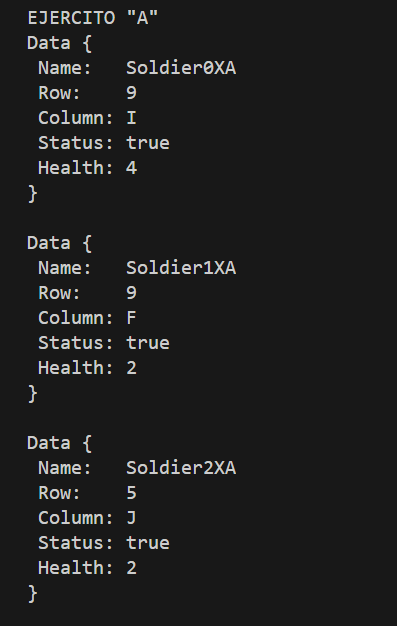
\includegraphics[width=0.5\textwidth,keepaspectratio]{img/toString.png}
            \caption{}
        \end{figure}

        
        \begin{lstlisting}[language=bash,caption={Commit: En el primer commit se reutilizaba la clase Soldado.java del laboratorio anterior}][H]
    		$ git add .
    		$ git commit -m "Se reutilizo las clases del laboratorio anterior, para en este caso realizarlo con arraylist"			
    		$ git push -u origin main
    	\end{lstlisting}
     
        %%%%%%%%%%%%%%%%
        
        \subsubsection{Clase VideoJuego.java}

        \begin{itemize}
            \item Primero se comenzó con la creación de la clase. 
            \item Posterior a ello se crearon dos variables de clase: 
            \begin{itemize}
                \item Un ArrayList bidimensional, el cual contendrá a los soldados del ejército.
                \item Además de un ArrayList unidimensional que nos servirá para contener a los soldados creados previamente, de esta manera será más fácil trabajar con ellos en los futuros métodos.
            \end{itemize}
        \end{itemize}

        \lstinputlisting[language=Java, firstline=7, lastline=10,firstnumber=7,numbers=left]{src/VideoJuego3.java}
    
        %%%%%%%%%%%%%%%%
        \subsubsection{Método para la creación de los ejército}

        \begin{itemize}
            \item El método tiene como nombre \textcolor{blue}{createArmy()}.
            \item Primero se define el número de soldados que contendrá cada ejército, haciendo uso de \textcolor{blue}{Math.random}.
            \item Luego utilizando un doble bucle for, se inicializa el ArrayList bidimensional de soldados en \textcolor{blue}{null}.
            \item Ahora se llama dos veces al método \textcolor{blue}{createArmyTeam} para realizar la creación de los dos ejércitos a partir de los tamaños ya establecidos anteriormente.
        \end{itemize}

        \lstinputlisting[language=Java, firstline=55, lastline=67,firstnumber=55,numbers=left]
        {src/VideoJuego3.java}
        
        \begin{lstlisting}[language=bash,caption={Commit: Se implementó el método createArmy()}][H]
    		$ git add .
    		$ git commit -m "Se realizaron modificaciones para que ahora el programa trabaje con 2 ejercitos, se adapto el metodo createArmy con la ayuda de otro metodo que trabajara con cada ejercito llamado createArmyTeam"			
    		$ git push -u origin main
    	\end{lstlisting}
        
        %%%%%%%%%%%%%%%%
        \subsubsection{Método para la creación de ejércitos}

        \begin{itemize}
            \item El método tiene como nombre \textcolor{blue}{createArmyTeam()}.
            \item Recibe como parámetros un entero que es el número de soldados del ejército, el ArrayList de soldados a utilizar y un String que es el char que va al final del nombre de los soldados, esto último nos ayuda a identificarlos mejor.
            \item Utilizando un do while se crean posiciones aleatorias en el ArrayList bidimensional, tomando como condición que dicha posición sea distinta de \textcolor{blue}{null}.
            \item Finalmente se crea el soldado, se almacena en ambos arreglos y retorna el ArrayList unidimensional con los soldados creados.

        \end{itemize}
        
        \lstinputlisting[language=Java, firstline=69, lastline=83,firstnumber=69,numbers=left]
        {src/VideoJuego3.java}

        %%%%%%%%%%%%%%%%
        
        \subsubsection{Método para mostrar la tabla con el ejército}

        \begin{itemize}
            \item El método tiene como nombre \textcolor{blue}{showArmyTable()}.
            \item La funcionalidad es simple:
            \begin{itemize}
                \item Se crean dos String (\textcolor{blue}{linesUp, linesDown}), estos son usados para la impresión.
                \item Primeramente se imprime la parte superior, donde se encuentran las letras que indica las columnas. Seguido de una linea que representa la parte superior de la tabla.
                \item Se utilizó dos bucles for, el primero para las filas y el segundo para las columnas.
                \item En el primero, inicia imprimiendo linesUp y luego de un salto de línea imprime el número de fila, se agregó una condicional que nos sirve para darle un toque de simetría a esta enumeración de fila, y así evitar que al momento de imprimir el 10 recorra un espacio.
                \item Dentro del segundo, se evalúa si contiene un Soldado o \textcolor{blue}{\texttt{null}}; en caso de ser así, imprimirá \textcolor{violet}{`` |''}, en caso de contener a un soldado completará el cuadrado de la tabla incluyendo ejército (A o B), y su nombre simplificado (S + número generado).
                \item Finalmente se imprime linesDown que completaría la línea inferior de cada fila.
            \end{itemize}
        \end{itemize}

        \lstinputlisting[language=Java, firstline=85, lastline=102,firstnumber=85,numbers=left]{src/VideoJuego3.java}

        \begin{itemize}
            \begin{itemize}
                \item Un ejemplo de como se muestra en la siguiente imagen:
            \end{itemize}
        \end{itemize}

        \begin{figure}[H]
            \centering
            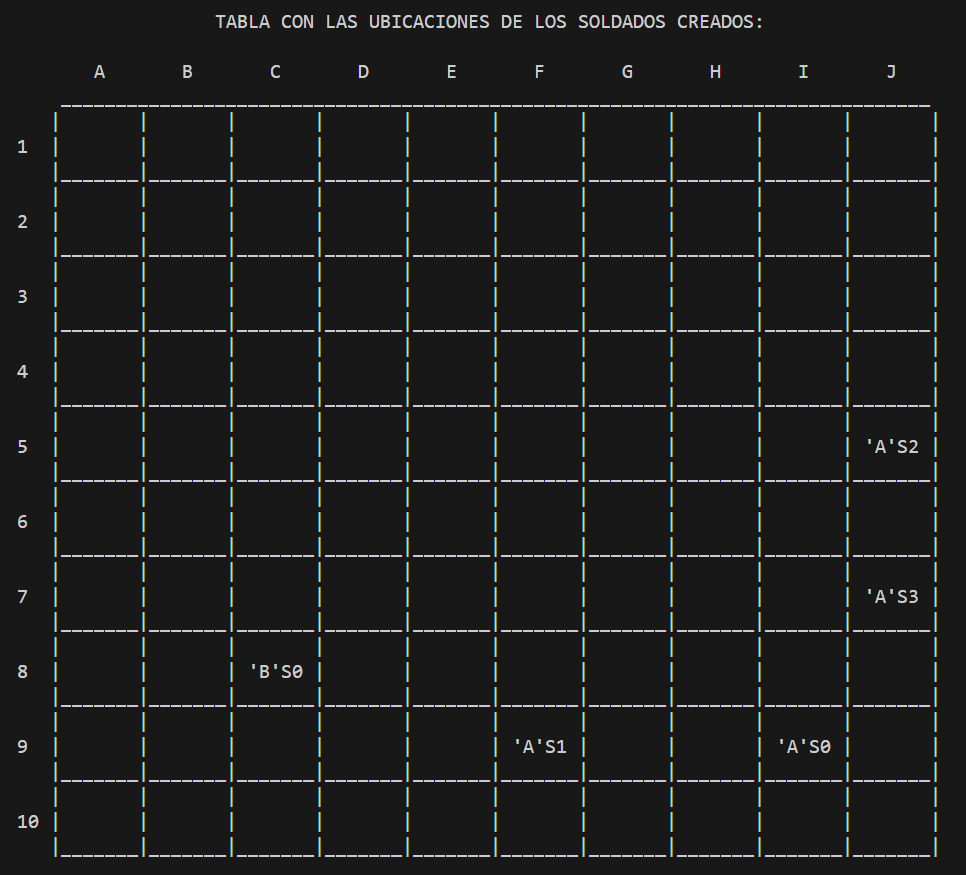
\includegraphics[width=0.7\textwidth,keepaspectratio]{img/showArmyTable.png}
            \caption{}
        \end{figure}

        \begin{lstlisting}[language=bash,caption={Commit: Se adaptó e implementó el método para mostrar la tabla con los soldados de ambos ejércitos}][H]
    		$ git add .
    		$ git commit -m "Se modifico el metodo showArmyTable, con ayuda de un metodo que sirve al momento de graficar, este verifica a que team pertenece y segun eso sera mostrado en la tabla"
    		$ git push -u origin main
    	\end{lstlisting}
        
        %%%%%%%%%%%%%%%%
        
        \subsubsection{Método para verificar si pertenece a un ejército}

        \begin{itemize}
            \item El método tiene como nombre \textcolor{blue}{isTeam()}.
            \item Simplemente dentro del método se recorrerá el ArrayList de soldados, en cada iteración se evaluará si pertenece al ejército dado.
            \item En caso se encuentre uno igual, se retornará \textcolor{blue}{true}, y si es que termina el bucle for y no encontró ninguno, retornará \textcolor{blue}{false}.
        \end{itemize}

        \lstinputlisting[language=Java, firstline=104, lastline=109,firstnumber=104,numbers=left]{src/VideoJuego3.java}
        
        %%%%%%%%%%%%%%%%
        
        \subsubsection{Método para mostrar los datos de los soldados de un ejército}

        \begin{itemize}
            \item El método tiene como nombre \textcolor{blue}{showArmyData()}.
            \item Este usa un for each para recorrer el arreglo unidimensional de Soldado, y luego mostrar sus datos con el System.out.println, que a su vez este sigue el formato que se estableció en el método \textcolor{blue}{toString()} de la clase Soldado.java.
            \item La impresión en consola será la misma que la figura 1.
        \end{itemize}

        \lstinputlisting[language=Java, firstline=111, lastline=114,firstnumber=111,numbers=left]{src/VideoJuego3.java}

        \begin{lstlisting}[language=bash,caption={Commit: Se adaptó e implementó el método para mostrar los datos de los soldados de un ejército}][H]
    		$ git add .
    		$ git commit -m "Se cambio el parametro del metodo showArmyData a un ArrayList, de esta manera recibira los ArrayList de ambos ejercitos"
    		$ git push -u origin main
    	\end{lstlisting}
        
        %%%%%%%%%%%%%%%%
        
        \subsubsection{Método para mostrar aquellos soldados con más vida de un ejército}
        
        \begin{itemize}
            \item El método tiene como nombre \textcolor{blue}{moreHealt()}.
            \item Primero recorre el ArrayList unidimensional de soldados haciendo uso de un bucle for, de esta manera obtendrá el máximo de vida del ejército, el cual será almacenado en un entero maxHealth.
            \item Finalmente imprimirá aquellos soldados que tengan la vida igual a maxHealth, con un for y un if que controlará aquello.

        \end{itemize}

        \lstinputlisting[language=Java, firstline=116, lastline=126,firstnumber=116,numbers=left]{src/VideoJuego3.java}

        \begin{itemize}
            \begin{itemize}
                \item Un ejemplo de como se muestra en la siguiente imagen:
            \end{itemize}
        \end{itemize}

        \begin{figure}[H]
            \centering
            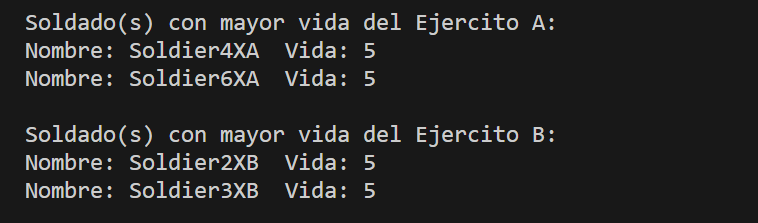
\includegraphics[width=0.7\textwidth,keepaspectratio]{img/moreHealth.png}
            \caption{}
        \end{figure}

        \begin{lstlisting}[language=bash,caption={Commit: Se agregó el método moreHealt() que imprimirá aquellos soldados que tengan la mayor vida dentro de su ejército}][H]
    		$ git add .
    		$ git commit -m "Se adapto el metodo moreHealth para trabajar con los ArrayList de soldados, este sera aplicado para cada ejercito"
    		$ git push -u origin main
    	\end{lstlisting}
        
        %%%%%%%%%%%%%%%%
        \newpage
        \subsubsection{Método para hallar la suma de vida en un ejército}

        \begin{itemize}
            \item El método tiene como nombre \textcolor{blue}{sumHealth()}.
            \item Se utiliza un entero inicializado en 0 para mientras que se recorre el arreglo unidimensional de Soldado con un bucle for each, este entero (sum) va almacenando la vida de todos los soldados.
            \item Finalmente se retorna \textcolor{blue}{sum} para que sea utilizado en el main.
        \end{itemize}

        \lstinputlisting[language=Java, firstline=132, lastline=137,firstnumber=93,numbers=left]{src/VideoJuego3.java}

        \begin{itemize}
            \begin{itemize}
                \item Un ejemplo de como se muestra en la siguiente imagen:
            \end{itemize}
        \end{itemize}

        \begin{figure}[H]
            \centering
            
\includegraphics[width=0.7\textwidth,keepaspectratio]{img/sumHealth.png}
            \caption{}
        \end{figure}

        \begin{figure}[H]
            \centering
            
\includegraphics[width=0.7\textwidth,keepaspectratio]{img/sumHealth2.png}
            \caption{}
        \end{figure}
        
        %%%%%%%%%%%%%%%%
        
        \subsubsection{Método para hallar el promedio de vida en un ejército}

        \begin{itemize}
            \item El método tiene como nombre \textcolor{blue}{averageHealth()}.
            \item De manera breve como el método, este retorna una división entre la suma de la vida del ejército, haciendo uso del método \textcolor{blue}{sumHealth()} y dividiendo entre el tamaño del ejército.
        \end{itemize}

        \lstinputlisting[language=Java, firstline=128, lastline=130,firstnumber=128,numbers=left]{src/VideoJuego3.java}

        \begin{itemize}
            \begin{itemize}
                \item Un ejemplo de como se muestra en la siguiente imagen:
            \end{itemize}
        \end{itemize}

        \begin{figure}[H]
            \centering
            
\includegraphics[width=0.7\textwidth,keepaspectratio]{img/averageHealth.png}
            \caption{}
        \end{figure}

        \begin{figure}[H]
            \centering
            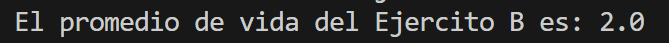
\includegraphics[width=0.7\textwidth,keepaspectratio]{img/averageHealth2.png}
            \caption{}
        \end{figure}
        
        %%%%%%%%%%%%%%%%
        \newpage
        \subsubsection{Método de ordenamiento BubbleSort}

        \begin{itemize}
            \item El método tiene como nombre \textcolor{blue}{bubbleSort()}.
            \item El método tiene como finalidad ordenar el ArrayList unidimensional de Soldado haciendo uso del algoritmo BubbleSort, tomando en cuenta la vida de los soldados que contiene dicho ArrayList. Este algoritmo se extrajo de Geeksforgeeks y fue adaptado a este proyecto.
        \end{itemize}

        \lstinputlisting[language=Java, firstline=139, lastline=156,firstnumber=139,numbers=left]{src/VideoJuego3.java}

        \begin{lstlisting}[language=bash,caption={Commit: Se implementó el método bubbleSort() para ordenar los soldados de mayor a menor vida}][H]
    		$ git add .
    		$ git commit -m "Se adapto el algoritmo de ordenamiento en el metodo bubbleSort para trabajar ahora con los ArrayList de soldados"			
    		$ git push -u origin main
    	\end{lstlisting}
        
        %%%%%%%%%%%%%%%%
        \newpage
        \subsubsection{Método de ordenamiento InsertionSort}
        
        \begin{itemize}
            \item El método tiene como nombre \textcolor{blue}{insertionSort()}.
            \item El método tiene como finalidad ordenar el ArrayList unidimensional de Soldado haciendo uso del algoritmo InsertionSort, tomando en cuenta la vida de los soldados que contiene dicho ArrayList. Este algoritmo se extrajo de Geeksforgeeks y fue adaptado a este proyecto.
        \end{itemize}
        
        \lstinputlisting[language=Java, firstline=158, lastline=173,firstnumber=158,numbers=left]{src/VideoJuego3.java}

        \begin{lstlisting}[language=bash,caption={Commit: Se implementó el método insertionSort()}][H]
    		$ git add .
    		$ git commit -m "Se adapto el metodo insertionSort para ordenar los ArrayList de soldados"
    		$ git push -u origin main
    	\end{lstlisting}
        
        %%%%%%%%%%%%%%%%
        \newpage
        \subsubsection{Método de ordenamiento SelectionSort}

        \begin{itemize}
            \item El método tiene como nombre \textcolor{blue}{selectionSort()}.
            \item El método tiene como finalidad ordenar el ArrayList unidimensional de Soldado haciendo uso del algoritmo SelectionSort, tomando en cuenta la vida de los soldados que contiene dicho ArrayList. Este algoritmo se extrajo de Geeksforgeeks y fue adaptado a este proyecto.
        \end{itemize}

        \lstinputlisting[language=Java, firstline=175, lastline=191,firstnumber=175,numbers=left]{src/VideoJuego3.java}

        \begin{lstlisting}[language=bash,caption={Commit: Se implementó el método selectionSort()}][H]
    		$ git add .
    		$ git commit -m "Se adapto el metodo selectionSort el cual es nuestro ultimo metodo de algoritmo de ordenamiento para que trabaje con ArrayList de soldados"			
    		$ git push -u origin main
    	\end{lstlisting}
        
        %%%%%%%%%%%%%%%%
        \newpage
        \subsubsection{Método para imprimir los soldados de un ejército, ordenados según su vida}
        
        \begin{itemize}
            \item El método tiene como nombre \textcolor{blue}{printArmyHealth()}.
            \item Este método recibirá un ArrayList unidimensional de Soldado (previamente ordenado), lo recorrerá usando un bucle for y mostrará los soldados, teniendo en cuenta que primero se mostrarán los de mayor vida hasta los de menor.
        \end{itemize}
        
        \lstinputlisting[language=Java, firstline=193, lastline=196,firstnumber=193,numbers=left]{src/VideoJuego3.java}

        \begin{lstlisting}[language=bash,caption={Commit: Se implementaró el método showArmyHealth}][H]
    		$ git add .
    		$ git commit -m "Se adapto el metodo printArmy cambiandole el parametro y el metodo que accede al ArrayList, para de esta manera trabajar con los mismo"	
    		$ git push -u origin main
    	\end{lstlisting}

        \begin{itemize}
            \begin{itemize}
                \item Un ejemplo de como se muestra utilizando los 3 algoritmos de ordenamiento en la siguiente imagen:
            \end{itemize}
        \end{itemize}

        \begin{figure}[H]
            \centering
            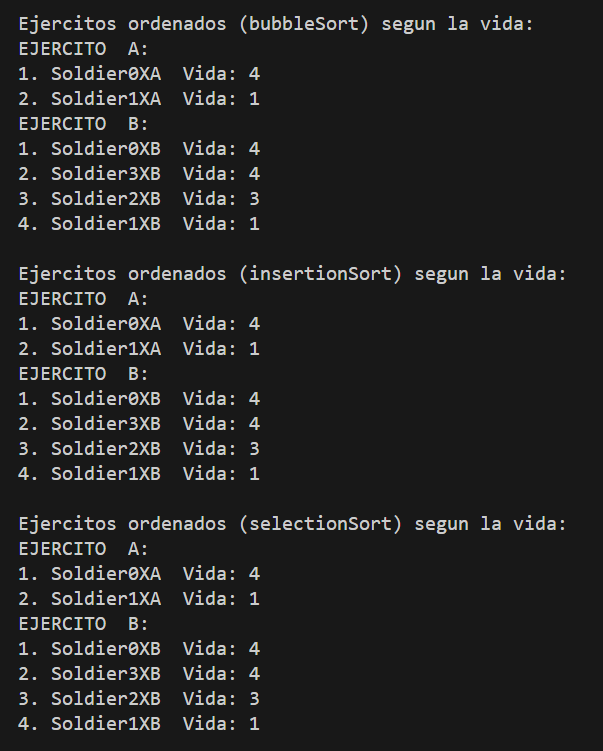
\includegraphics[width=0.5\textwidth,keepaspectratio]{img/printArmyHealth.png}
            \caption{}
        \end{figure}
        
        %%%%%%%%%%%%%%%%
        
        \subsubsection{Método para mostrar al ejército ganador según la vida de sus soldados}
        
        \begin{itemize}
            \item El método tiene como nombre \textcolor{blue}{armyWinnerHealth()}.
            \item Este método utilizará la suma de vida de cada ejército, hará comparaciones y si uno de los dos es superior en número de vida, se imprimirá que ganó, en caso de ser iguales mostrará aquello.
        \end{itemize}
        
        \lstinputlisting[language=Java, firstline=198, lastline=207,firstnumber=198,numbers=left]{src/VideoJuego3.java}

        \begin{lstlisting}[language=bash,caption={Commit: Se implementaró el método armyWinnerHealth}][H]
    		$ git add .
    		$ git commit -m "Se implemento un metodo armyWinnerHealth, este mostrara al ganador en caso de una batalla, la cual da como ganador al que tenga la mayor suma de vida en soldados"	
    		$ git push -u origin main
    	\end{lstlisting}
        
        %%%%%%%%%%%%%%%%
        \subsubsection{Método main, utilización de los métodos creados}
        
        \begin{itemize}
            \item En el método principal (main) se utilizarán los métodos creados anteriormente para cumplir con lo pedido en el trabajo.
            \item Primero llenaremos los ArrayList army1DA y army1DB haciendo uso del método \textcolor{blue}{createArmy()} que a su vez inicializará el arreglo bidimensional de soldados.
            \item Luego usaremos el método \textcolor{blue}{showArmyData()} para mostrar los soldados creados, siguiendo ese mismo orden, esto para ambos ejércitos (A y B).
            \item Seguido se llamará al método showArmyTable para mostrar la tabla con los soldados ubicados en la misma.
            \item Seguidamente se llama al método \textcolor{blue}{moreHealth()}, este nos mostrará aquellos que tengan la mayor vida de cada ejército.
            \item Para mostrar la suma y promedio de vida en nuestros ejércitos, se utiliza los métodos \textcolor{blue}{sumHealth()} y \textcolor{blue}{averageHealth()} respectivamente, para luego ser mostrados en consola.
            \item Finalmente haciendo uso de los 3 métodos que contienen los algoritmos de ordenamiento(\textcolor{blue}{bubbleSort(), insertionSort(), selectionsort()}), además del método \textcolor{blue}{printArmyHealth()} para mostrar los ejércitos ordenados según la vida, utilizando cada uno siguiendo el orden mencionado de nuestros algoritmos.
        \end{itemize}
        \newpage
        \lstinputlisting[language=Java, firstline=11, lastline=53,firstnumber=11,numbers=left]{src/VideoJuego3.java}
        
        %%%%%%%%%%%%%%%%
        
        \begin{lstlisting}[language=bash,caption={Commit: Último commit, donde se cambió el nombre de la clase a el pedido en el trabajo, el cual es: VideoJuego3.java}][H]
    		$ git add .
    		$ git commit -m "Cambiando el nombre de la clase, pasa de ser DemoBatalla a VideoJuego3"
    		$ git push -u origin main
    	\end{lstlisting}

    
%-----------------------------------------------------------------------------------
%------------------------------ ESTRUCTURA DE LABORATORIO --------------------------
%-----------------------------------------------------------------------------------
    \newpage
	\subsection{Estructura de laboratorio 06}
    \begin{itemize}	
		\item El contenido que se entrega en este laboratorio es el siguiente:
	\end{itemize}
	
\begin{lstlisting}[style=ascii-tree]

    lab05
    |   VideoJuego3.java
    |   Soldado.java
    |
    |───latex
        |   Informe_Lab06.pdf
        |   Informe_Lab06.tex
        |
        |───img
        |       averageHealth.png
        |       averageHealth2.png
        |       logo_abet.png
        |       logo_episunsa.png
        |       logo_unsa.jpg
        |       moreHealth.png
        |       printArmyHealth.png
        |       showArmyTable.png
        |       sumHealth.png
        |       sumHealth2.png
        |       toString.png
        |
        |───src
                Soldado.java
                VideoJuego3.java

\end{lstlisting}    

	\section{\textcolor{red}{Rúbricas}}
	
	\subsection{\textcolor{red}{Entregable Informe}}
	\begin{table}[H]
		\caption{Tipo de Informe}
		\setlength{\tabcolsep}{0.5em} % for the horizontal padding
		{\renewcommand{\arraystretch}{1.5} % for the vertical padding
		\begin{tabular}{|p{3cm}|p{12cm}|}
			\hline
			\multicolumn{2}{|c|}{\textbf{\textcolor{red}{Informe}}}  \\
			\hline 
			\textbf{\textcolor{red}{Latex}} & \textcolor{blue}{El informe está en formato PDF desde Latex,  con un formato limpio (buena presentación) y fácil de leer.}   \\ 
			\hline 
			
			
		\end{tabular}
	}
	\end{table}
	
	\clearpage
%-----------------------------------------------------------------------------------
%------------------------------ RÚBRICA DE EVALUACIÓN ------------------------------
%-----------------------------------------------------------------------------------
 
	\subsection{\textcolor{red}{Rúbrica para el contenido del Informe y demostración}}
	\begin{itemize}			
		\item El alumno debe marcar o dejar en blanco en celdas de la columna \textbf{Checklist} si cumplió con el ítem correspondiente.
		\item Si un alumno supera la fecha de entrega,  su calificación será sobre la nota mínima aprobada, siempre y cuando cumpla con todos lo ítem.
		\item El alumno debe auto calificarse en la columna \textbf{Estudiante} de acuerdo a la siguiente tabla:
	
		\begin{table}[ht]
			\caption{Niveles de desempeño}
			\begin{center}
			\begin{tabular}{ccccc}
    			\hline
    			 & \multicolumn{4}{c}{Nivel}\\
    			\cline{1-5}
    			\textbf{Puntos} & Insatisfactorio 25\%& En Proceso 50\% & Satisfactorio 75\% & Sobresaliente 100\%\\
    			\textbf{2.0}&0.5&1.0&1.5&2.0\\
    			\textbf{4.0}&1.0&2.0&3.0&4.0\\
    		\hline
			\end{tabular}
		\end{center}
	\end{table}	
	
	\end{itemize}
	
	\begin{table}[H]
		\caption{Rúbrica para contenido del Informe y demostración}
		\setlength{\tabcolsep}{0.5em} % for the horizontal padding
		{\renewcommand{\arraystretch}{1.5}% for the vertical padding
		%\begin{center}
		\begin{tabular}{|p{2.7cm}|p{7cm}|x{1.3cm}|p{1.2cm}|p{1.5cm}|p{1.1cm}|}
			\hline
    		\multicolumn{2}{|c|}{Contenido y demostración} & Puntos & Checklist & Estudiante & Profesor\\
			\hline
			\textbf{1. GitHub} & Hay enlace URL activo del directorio para el  laboratorio hacia su repositorio GitHub con código fuente terminado y fácil de revisar. &2 &X &2 & \\ 
			\hline
			\textbf{2. Commits} &  Hay capturas de pantalla de los commits más importantes con sus explicaciones detalladas. (El profesor puede preguntar para refrendar calificación). &4 &X &3 & \\ 
			\hline 
			\textbf{3. Código fuente} &  Hay porciones de código fuente importantes con numeración y explicaciones detalladas de sus funciones. &2 &X &2 & \\ 
			\hline 
			\textbf{4. Ejecución} & Se incluyen ejecuciones/pruebas del código fuente  explicadas gradualmente. &2 &X &2 & \\ 
			\hline			
			\textbf{5. Pregunta} & Se responde con completitud a la pregunta formulada en la tarea.  (El profesor puede preguntar para refrendar calificación).  &2 &X &2 & \\ 
			\hline	
			\textbf{6. Fechas} & Las fechas de modificación del código fuente están dentro de los plazos de fecha de entrega establecidos. &2 &X &2 & \\ 
			\hline 
			\textbf{7. Ortografía} & El documento no muestra errores ortográficos. &2 &X &2 & \\ 
			\hline 
			\textbf{8. Madurez} & El Informe muestra de manera general una evolución de la madurez del código fuente,  explicaciones puntuales pero precisas y un acabado impecable.   (El profesor puede preguntar para refrendar calificación).  &4 &X &3 & \\ 
			\hline
			\multicolumn{2}{|c|}{\textbf{Total}} &20 & &18 & \\ 
			\hline
		\end{tabular}
		%\end{center}
		%\label{tab:multicol}
		}
	\end{table}
	
\clearpage

%------------------------------ REFERENCIAS ------------------------------

\section{Referencias}
\begin{itemize}			
    \item \url{https://docs.oracle.com/javase/tutorial/java/nutsandbolts/variables.html}
    \item \url{https://docs.oracle.com/javase/8/docs/api/java/util/ArrayList.html}
    \item \url{https://docs.oracle.com/javase/tutorial/java/javaOO/methods.html}
    \item \url{https://www.geeksforgeeks.org/selection-sort/}
    \item \url{https://www.geeksforgeeks.org/bubble-sort/}
    \item \url{https://www.geeksforgeeks.org/insertion-sort/}
    \item \url{https://es.stackoverflow.com/questions/108171/}
\end{itemize}	
	
%\clearpage
%\bibliographystyle{apalike}
%\bibliographystyle{IEEEtranN}
%\bibliography{bibliography}
			
\end{document}